\documentclass[spanish]{udpreport}
\usepackage[utf8]{inputenc}
\usepackage[spanish]{babel}
\documentclass{article}
\usepackage{graphicx}
\graphicspath{ {images/} 


\title{Laboratorio Nro. 3: Redes de Datos}
\author{Jose Miguel Reyes,Simon Oyaneder,Gonzalo Perez}
\date{13 de abril de 2016}

\begin{document}
\maketitle

\tableofcontents

\chapter{Introducción}
En este laboratorio aprendimos el uso de dos programas, el primero wireshark, que nos permitio analizar el trafico y decifrar los paquetes de una red, y el segundo scapy, el cual nos permitio crear paquetes de datos para probar en el hub y switch. 
\chapter{Desarrollo}
\section{Preguntas}

\subsection{¿Qué pasa cuando envió un paquete a la dirección FF:FF:FF:FF:FF:FF? ¿Quienes
lo reciben? ¿Por qué?}

Cuando enviamos paquetes con esa direccion los que recibieron la informacion fueron todos los computadores que estaban conectados a la red.\\\\
Esto ocurre ya que esa direccion MAC lo que hace es decirle a los dispositivos ya sea HUB o SWITCH que envie los paquetes a todos los que estan conectados en la red.

\subsection{¿Qué pasa cuando envió un paquete a una MAC de otro equipo? ¿Quienes lo
pueden reciben? ¿Por qué?}

Para poder responder esta pregunta y ser mas precisos la dividiremos en dos respuestas de acuerdo al equipo que este utilizandose.\\\\
En el caso del HUB, este hace que todos reciban el paquete pero que solo lo pueda ver el que tiene la MAC de destino, es de tipo broadcast.\\\\
Por otro lado en el SWITCH, este tiene otro funcionamiento el cual solo manda el paquete al que tiene la MAC de destino, es del tipo que llamamos unicast.

\subsection{¿Qué sucede si se envía un paquete a una MAC que no corresponda a ningún equipo
de la red? ¿Quienes lo pueden recepcionar? ¿Por qué?}

Igual que en la pregunta anterior  nos ponemos en el caso de los dos dispositivos que estamos usando. \\\\
Usando el HUB, el paquete llegara a todos los equipos de la red pero ninguno podra leerlo ya que la MAC de destino no es igual a ninguna de las MAC's de la red.\\\\
Por parte del SWITCH, este al ver que ninguna de las MAC's de los equipos en la red es igual al destinatario del paquete, no enviara el paquete por lo que ningun equipo lo recibira.



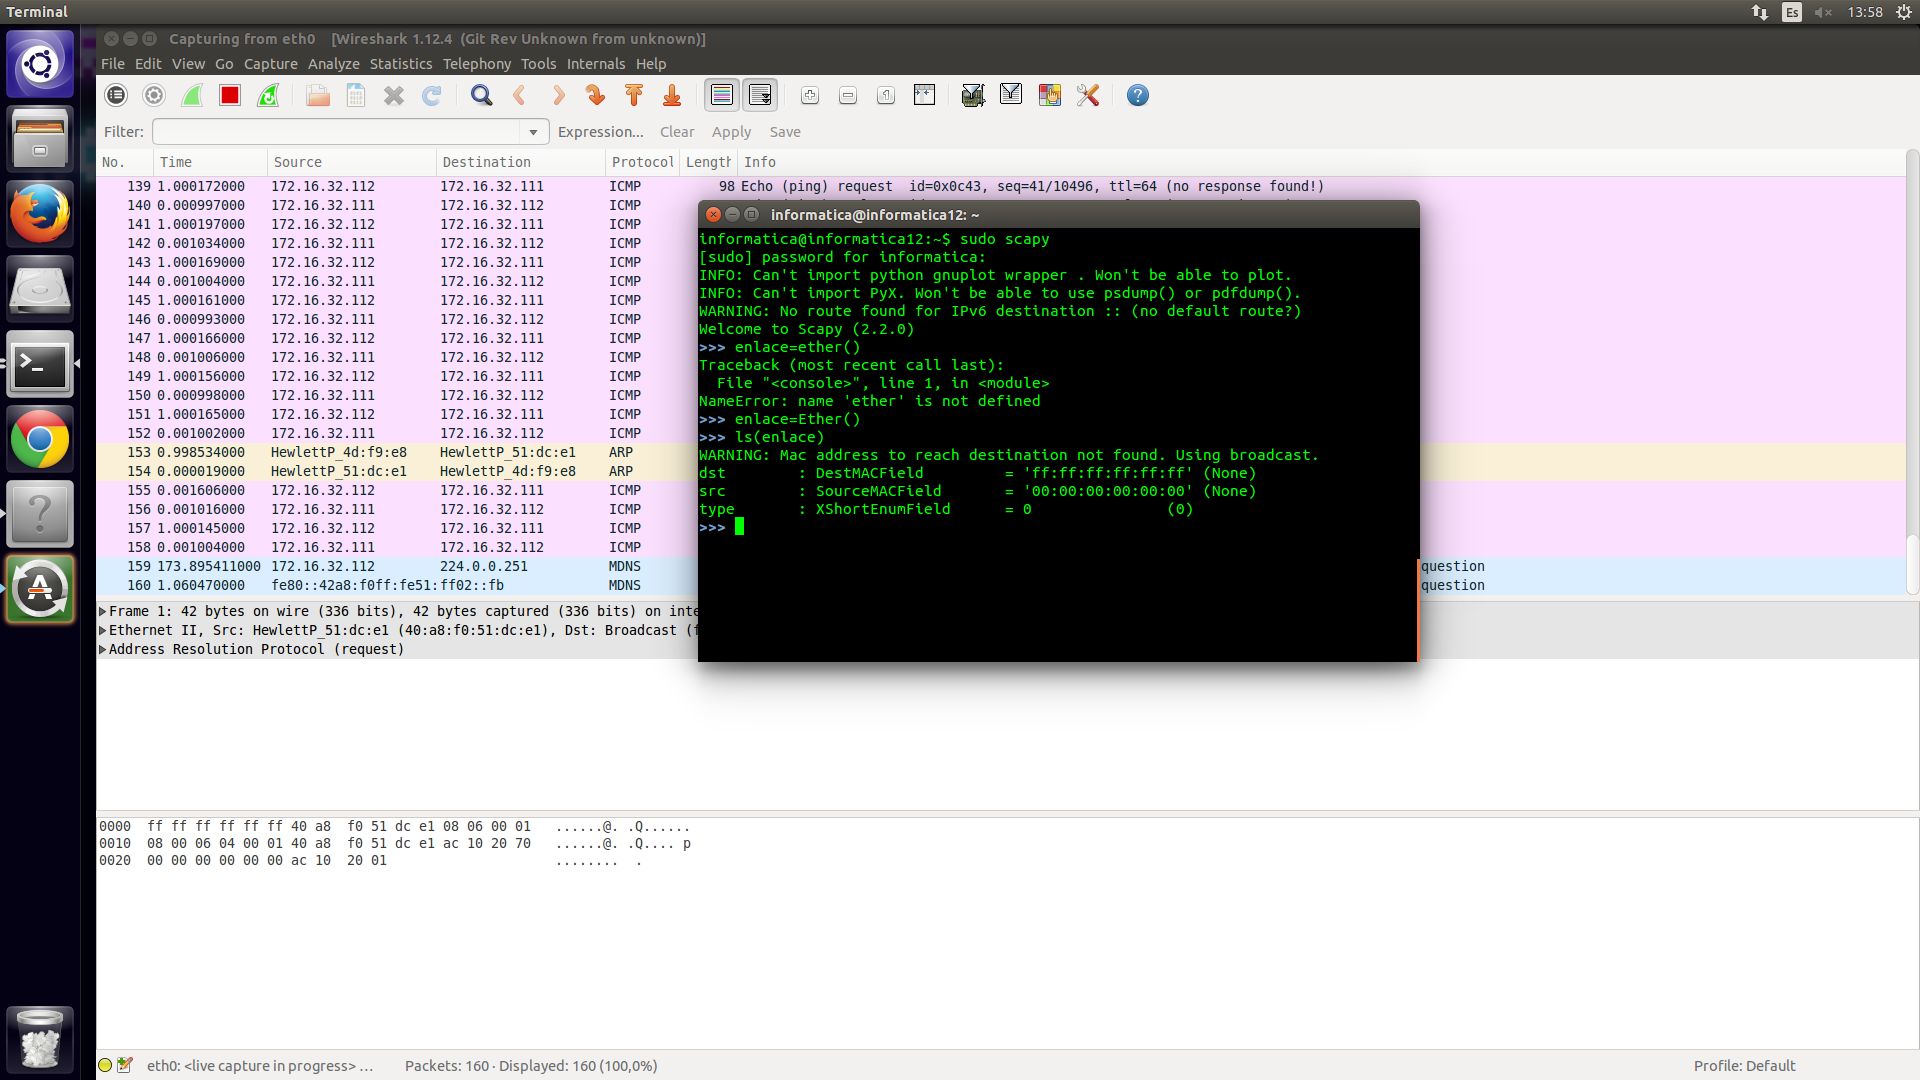
\includegraphics[scale=0.2]{fotos/1.png}


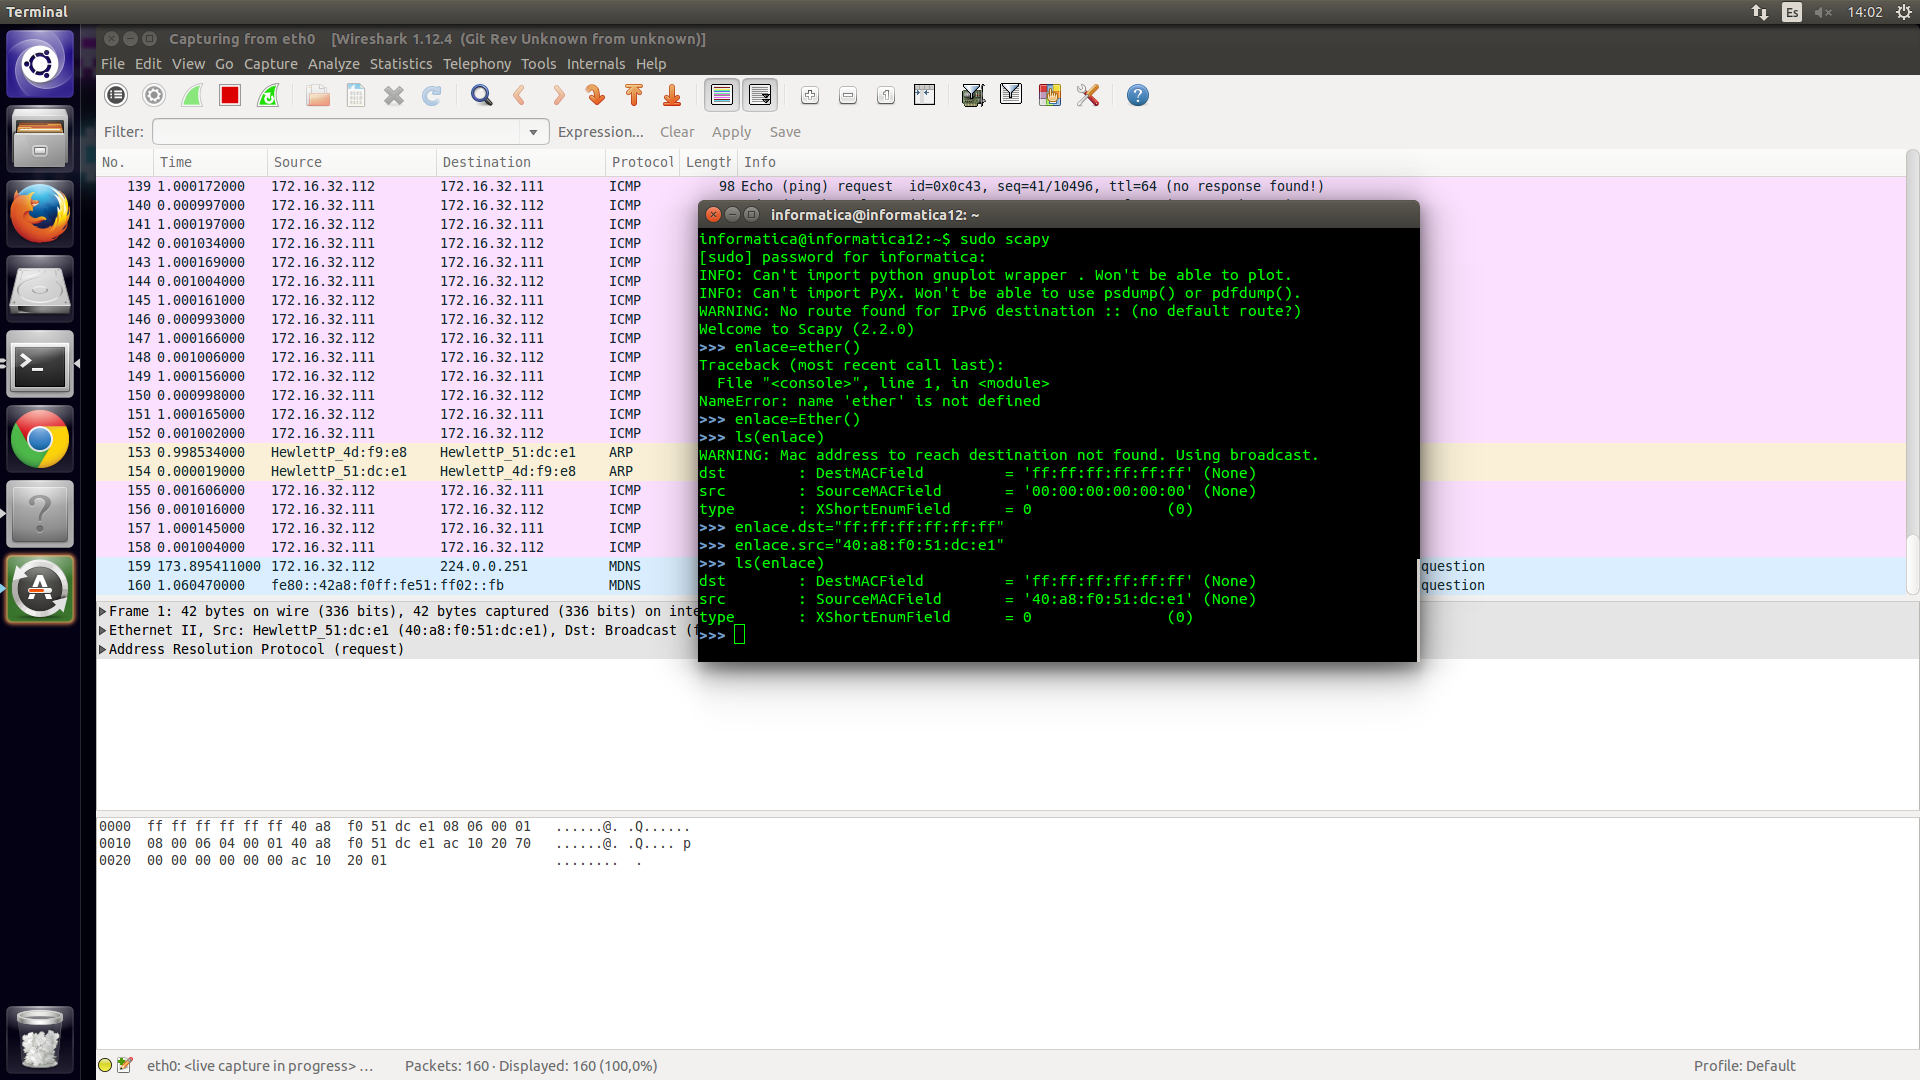
\includegraphics[scale=0.2]{fotos/2.png}


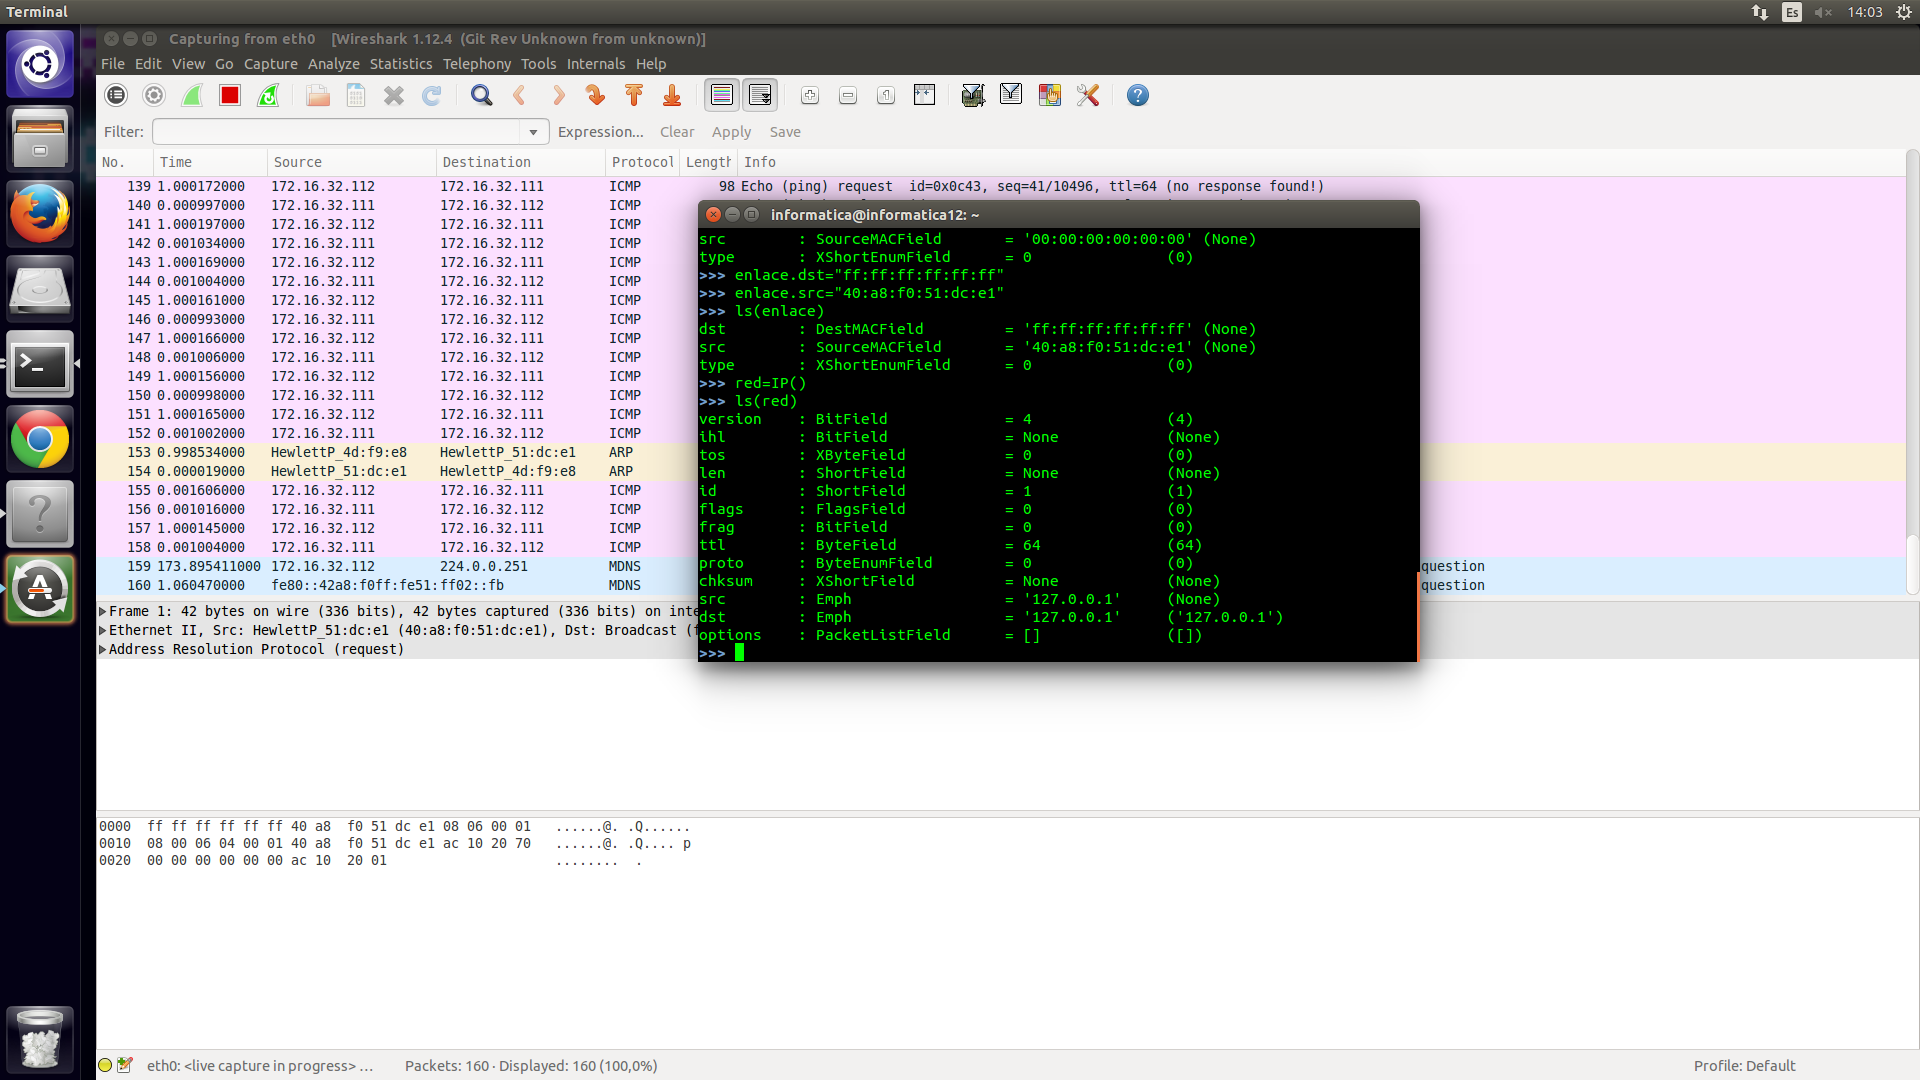
\includegraphics[scale=0.2]{fotos/3.png}


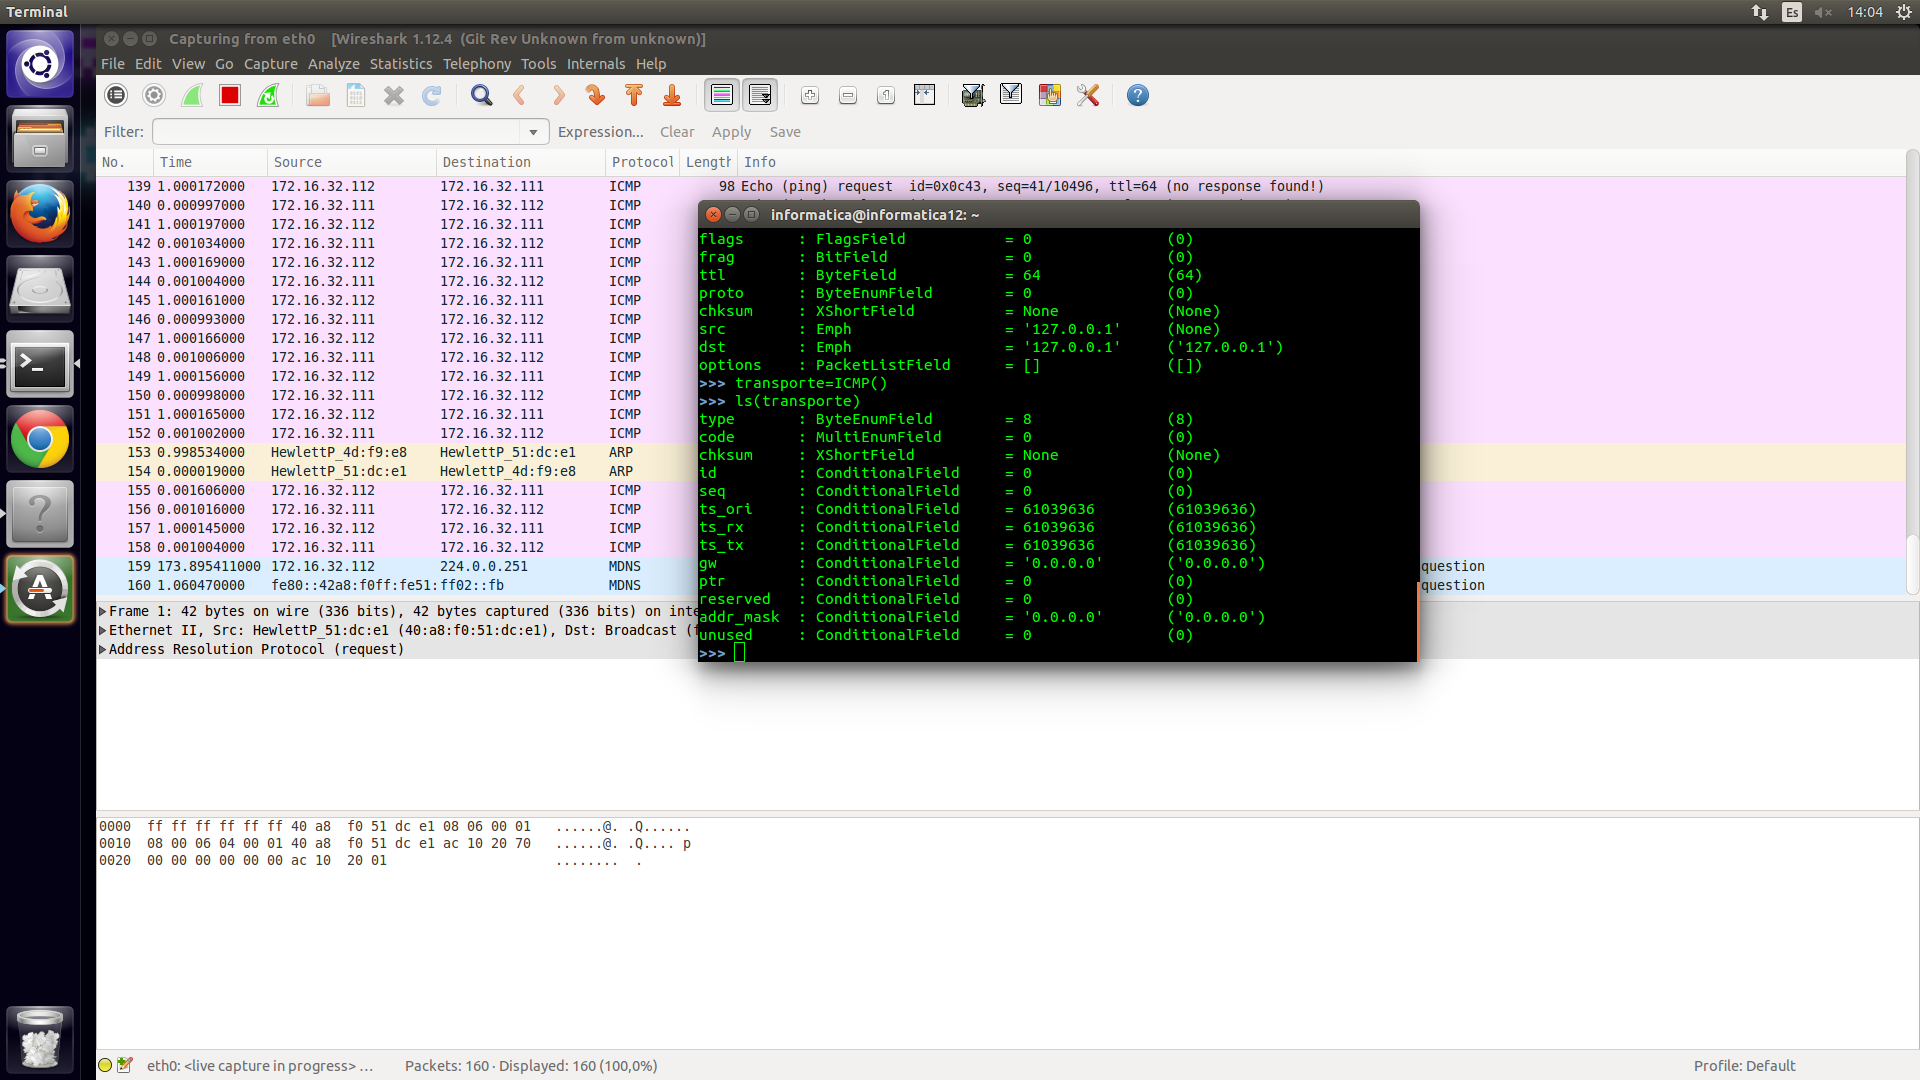
\includegraphics[scale=0.2]{fotos/4.png}


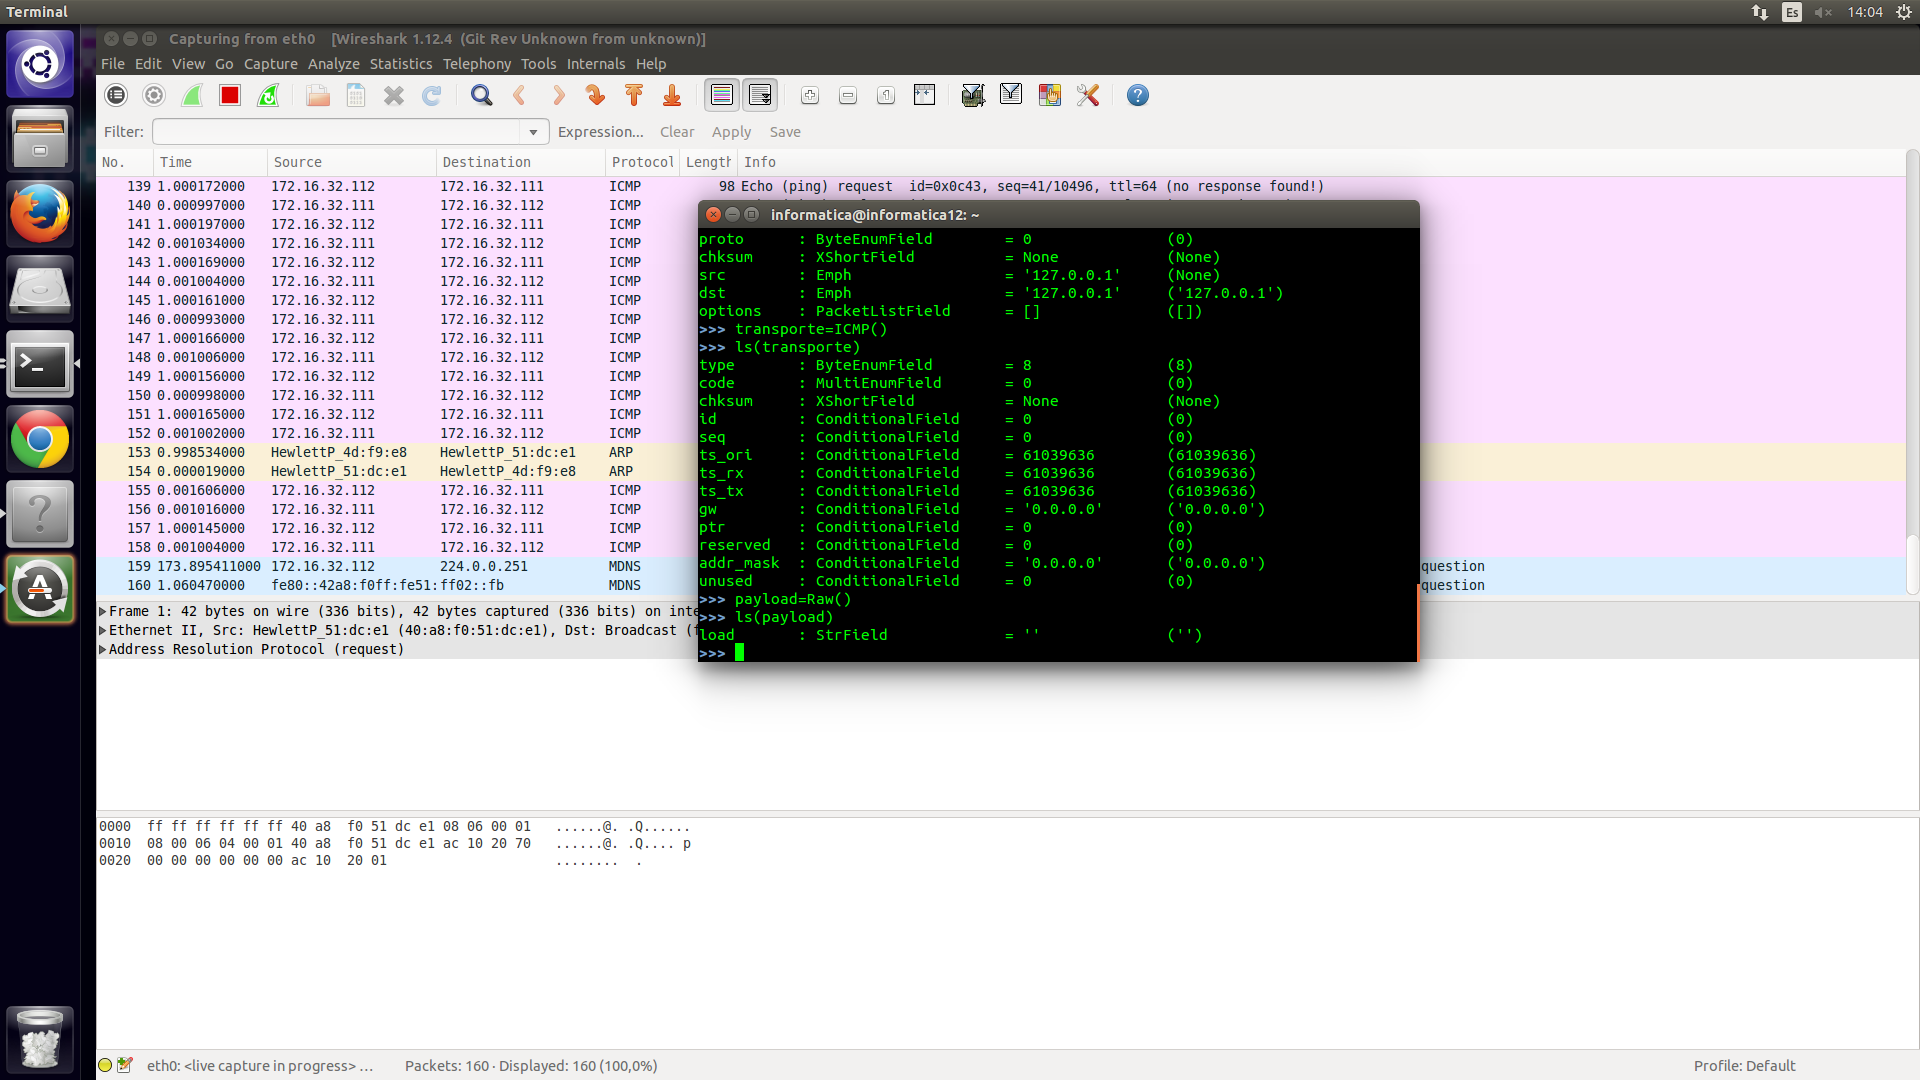
\includegraphics[scale=0.2]{fotos/5.png}


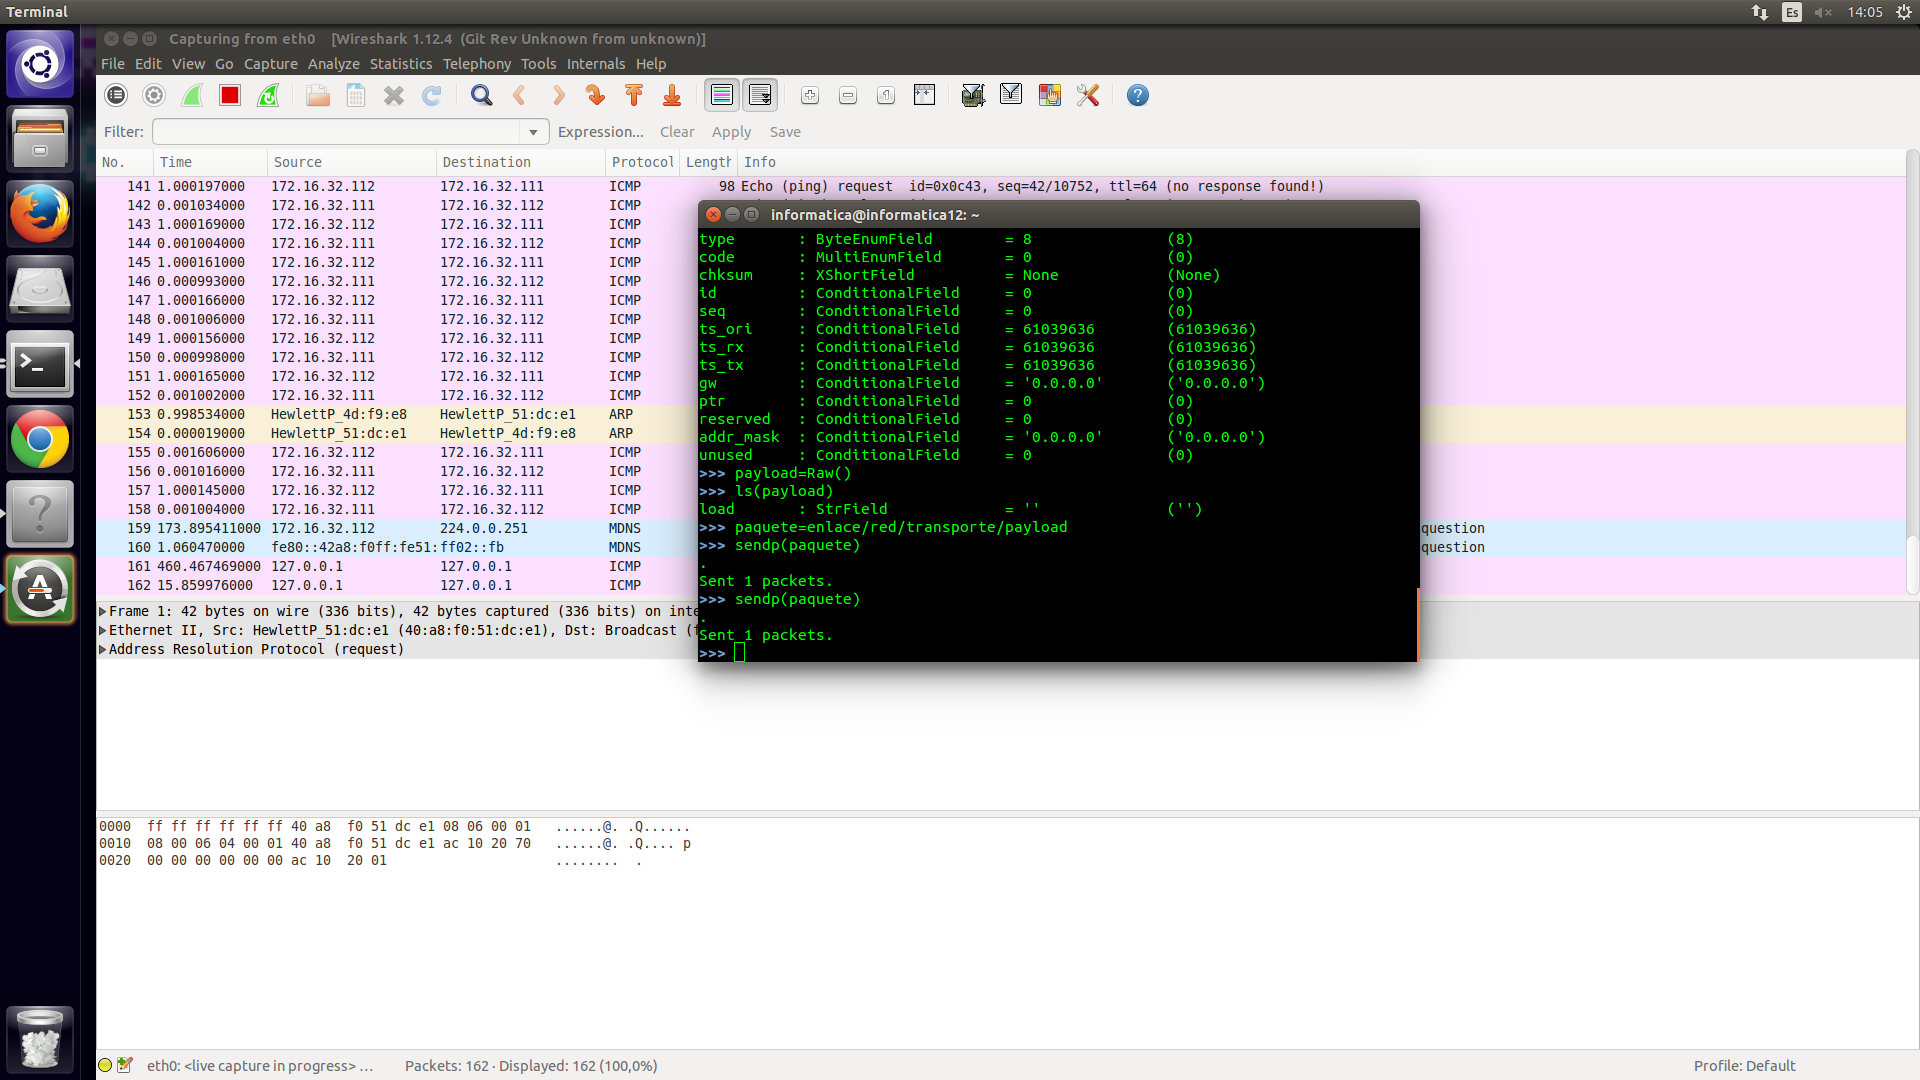
\includegraphics[scale=0.2]{fotos/6.png}


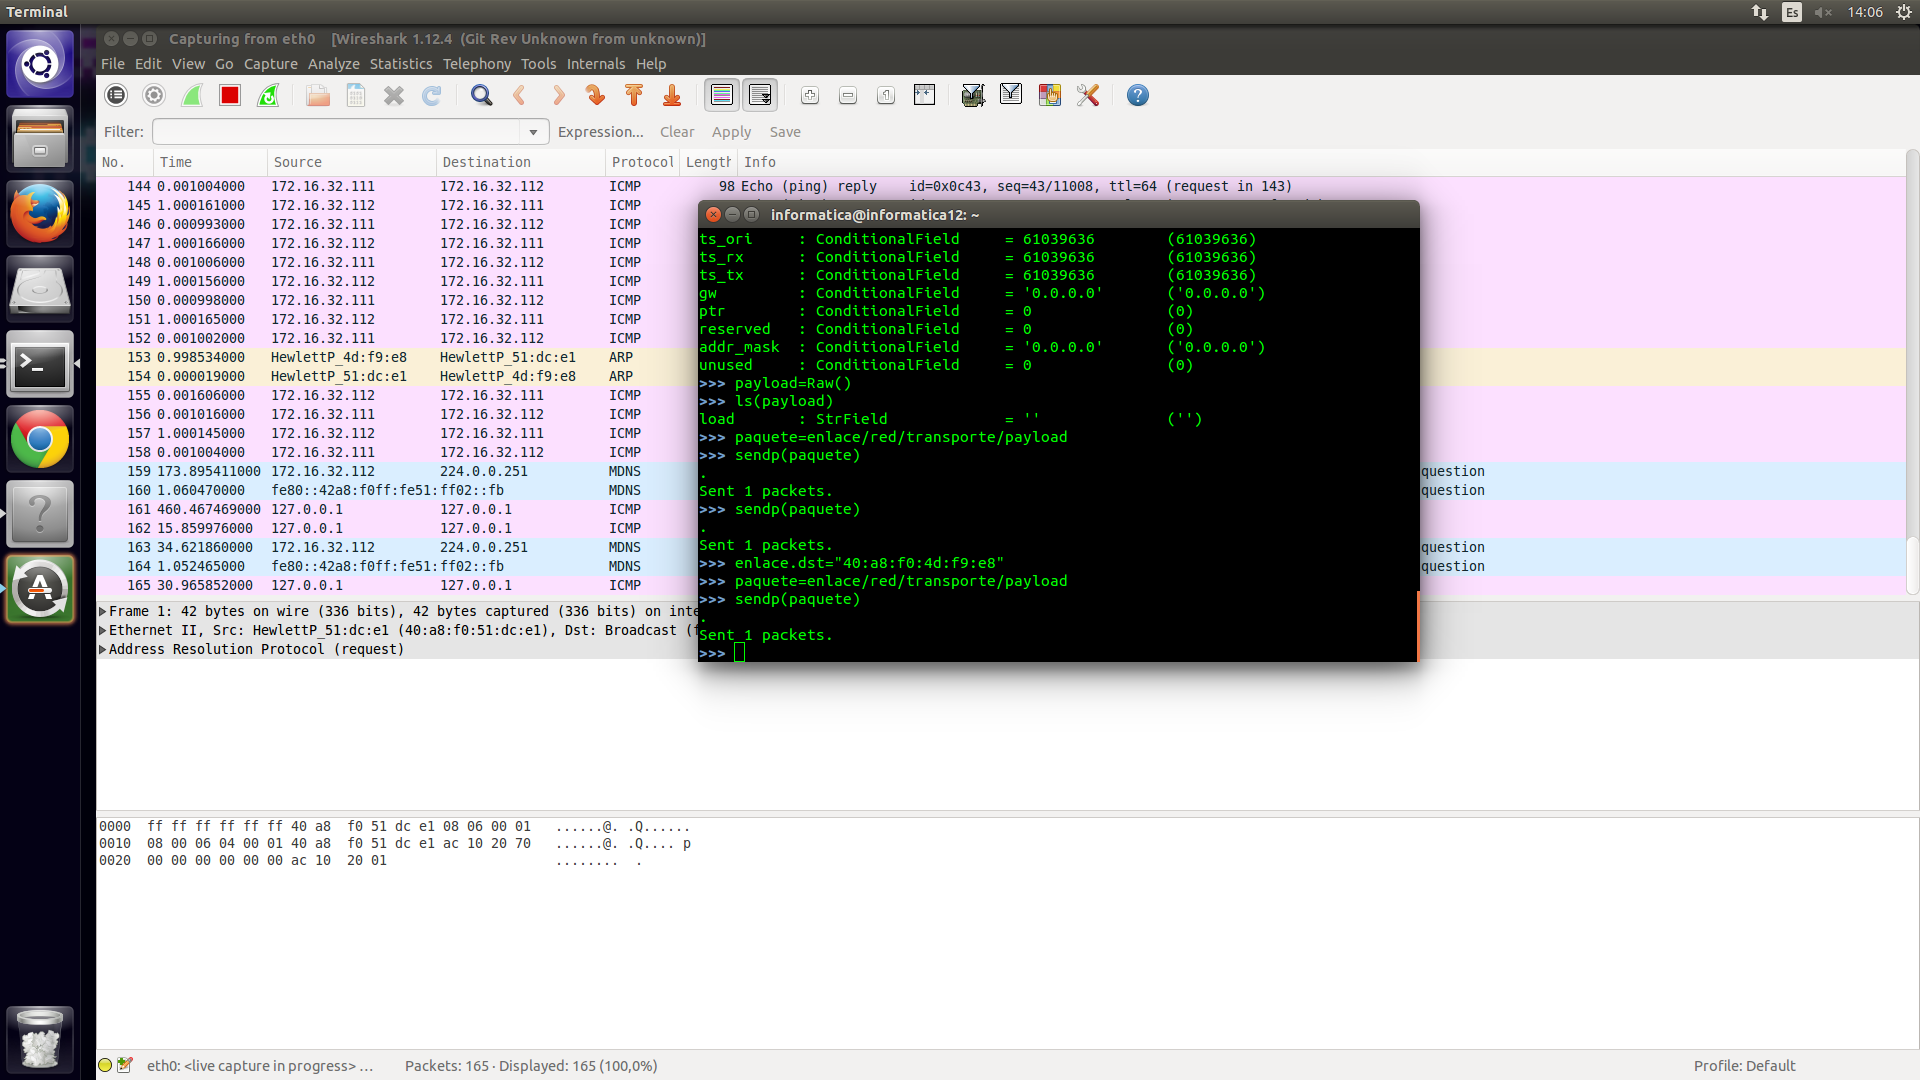
\includegraphics[scale=0.2]{fotos/8.png}


\chapter{Conclusión}
Despues de realizar este laboratorio pudimos apreciar el funcionamiento de diferentes equipos como lo son el HUB y el SWITCH. Ademas tambien vimos de forma practica el funcionamiento de las redes de tipo UNICAST y BROADCAST. Por otro lado nos permitio aprender la creacion y envio de paquetes y todo lo que hay que saber de una red basica.




\end{document}